% =====================================================================
% ANGLE 2 - THE COHORT FRONTIER  (self-contained draft for review)
% = existing "seafood disclosure frontier" chapter from main.tex,
%   PLUS a new theory framing (disclosure maturity + institutional convergence).
% =====================================================================
\section{5. The seafood disclosure frontier: evidence from six large
reporters}\label{cohort-analysis}

This chapter answers the thesis's second research question: \emph{what do mature
European seafood processors actually disclose?} It establishes that practice from
primary documents, setting the assumed \emph{upper bound} of sector disclosure
depth. Both the demand mapping that follows and the expectations placed on
smaller firms should be read against it. The cohort is not
a picture of typical practice; it is a picture of the best-in-class frontier.
This is Step~2 of the methodology set out in
Figure~\ref{fig:methodology-overview}.

\textbf{Scope note: this is a coverage analysis, not a judgement of reporting
quality.} It measures whether a topic is disclosed at all, coded from each
firm's own published sustainability report or ESRS-index appendix, using
only public information - no non-public data, site visits or firm-specific
verification. A firm scoring lower may simply have a different production
system, framework, or reporting year, not weaker sustainability performance;
no ranking or evaluative claim about the six companies is intended.

\FloatBarrier
\subsection{5.1 The frontier as a disclosure-maturity
question}\label{cohort-theory}

Corporate sustainability disclosure is not adopted all at once but develops
through stages of organisational maturity: firms move from ad-hoc, reactive
reporting toward systematic, integrated disclosure as capability accumulates
(Baumgartner \& Ebner, 2010),
and the completeness and quality of a firm's
reporting can be read as a position on that maturity gradient (C\"oster et al.,
2020).
The most advanced reporters in a sector therefore mark its practical
\emph{frontier}: the upper bound of what is currently feasible - and relevant to
seafood processing - to disclose given real data systems and resources. This research therefore treats the frontier as a ceiling that resource-constrained
SMEs can grow into, not one they can replicate today.

Two features make that frontier analytically useful here. First, when processors
as different as a vertically integrated salmon operation and a pure whitefish
processor nonetheless disclose the same handful of topics, that agreement is
unlikely to be coincidence. It reflects a shared expectation - what the sector
has collectively come to treat as standard practice for a credible reporter -
rather than each firm's independent choice; institutional theory calls this the
mimetic and normative pressure that makes practices converge across an industry
(DiMaggio \& Powell, 1983). This is an interpretive reading, and a competing one
is possible: firms may converge because the same topics carry the greatest
reputational risk, or simply because they are the easiest to report. That each
firm's disclosures are anchored in its own double-materiality assessment is a
partial check against pure convenience, though not a decisive one. Read either
way, a universal core is the sector's \emph{revealed} consensus on what a serious
reporter covers - what counts as complete disclosure in practice, not just a
coincidental overlap between six firms' independent choices.
Second, the frontier calibrates the realistic ambition for a
resource-constrained firm: if even the best-resourced reporters leave requirements
uncovered, completeness is the wrong yardstick for an SME, and the question
becomes which subset of disclosures matters most - the question the demand
mapping in the following chapter takes up.

Existing work characterises sustainability-reporting maturity in general terms
(Baumgartner \& Ebner, 2010) and describes seafood
sustainability governance at the level of the movement and its institutions (Bush
\& Oosterveer, 2019; Barclay \& Miller, 2018), but does not map, at
disclosure-requirement level, what the sector's leading firms actually report.
This chapter supplies that map and reads it for three things: how \emph{much} the
leading firms disclose (the height of the frontier), which topics \emph{every}
firm reports (the universal core), and which relevant topics \emph{none} of them
report (the sector's collective gaps).


\FloatBarrier
\subsection{5.2 The cohort and case selection}\label{cohort-selection}

Six large seafood processors were selected purposively as among the most
advanced sustainability reporters in the sector rather than as a
representative sample. The selection deliberately spans the sector's main
sourcing models, so that the disclosure pattern that emerges cannot be an
artefact of a single production system: wild-capture tuna (Thai Union,
Bolton), aquaculture salmon (Mowi), an integrated wild-plus-aquaculture
operation (Profand), and pure processing/branded firms whose variation comes
from the species and origins they source rather than from a distinct
production system of their own (Nomad Foods, Espersen).
All six are seafood \emph{processors}, but they differ in how far they integrate
upstream - from Mowi, which farms its own salmon and mills its own feed, to
Espersen, a near-pure whitefish processor. This matters for reading the
reports: Mowi discloses feed and farming as its \emph{own} operations,
while Espersen meets the same topics only as \emph{sourcing} questions about
its suppliers - the two are not directly comparable without accounting for
this difference.

The six were chosen on three criteria: they are among the largest seafood
processors by turnover; each publishes a full, structured sustainability report
under the ESRS or the GRI Standards; and together they span its main sourcing
models.

The second criterion carries most of the weight, and it is worth being precise
about what it does and does not establish. ``Most advanced'' here is a sampling
frame rather than a measured rank. Of the roughly 3{,}245 EU enterprises that
process fish as their main activity, about two-thirds are micro-enterprises and
only some two per cent employ 250 people or more (STECF, 2025). The
overwhelming majority therefore sit
below the CSRD reporting thresholds and face no obligation to publish a
structured sustainability report at all. Publishing one regardless is itself the
distinguishing act, and the six are drawn from the small population that does. No claim is made that they are the six \emph{best} reporters in the sector,
only that they sit inside the set that reports at all and, within it, span the
sourcing models and the size range.

Whether firms selected this way are advanced in absolute terms is a separate
question, and one this chapter's own results answer rather than assume. They are
not complete: the deepest reporter covers 60 of the 70 topical requirements and
the shallowest 33, and seven requirements are reported by no firm in the cohort
(Sections~5.4 and~5.6). The frontier they mark is therefore a realistic ceiling
rather than a standard of completeness - which is precisely why it is a usable
benchmark for a smaller firm.

The aim of the selection is therefore not representativeness but reach: to
assemble the firms most likely to have pushed disclosure to its current limit, so
that the pattern common to \emph{them} marks the sector's realistic ceiling.
By 2024 turnover the six span more than a tenfold range: Mowi (EUR~5.6bn) and
Thai Union (THB~138.4bn, approx. US\$4.0bn / EUR~3.6bn) are the largest, followed
by Bolton Group (EUR~3.5bn group-wide, of which approx. EUR~2.4bn is its food
division) and Nomad Foods (EUR~3.1bn), with Profand (approx. EUR~1.1bn) and
Espersen (DKK~3.3bn, approx. EUR~440m) smaller but still among the sector's
largest specialist processors.\footnote{2024 group turnover, most recent
published results, converted to EUR at approximate contemporaneous rates where
the firm did not report in EUR: Thai Union (\emph{Thai Union FY2024 press
release}, thaiunion.com); Mowi (\emph{Mowi Q4 2024 Report}, mowi.com); Bolton
Group (Undercurrent News, ``Tuna sales boost Bolton's turnover, profit in
2024,'' Aug.\ 2025); Nomad Foods (Q4/FY2024 earnings release, nomadfoods.com);
Profand (Undercurrent News, ``Spain's Profand surpasses EUR1bn revenue in
2024,'' Apr.\ 2025); Espersen (Undercurrent News / SeafoodSource coverage of
FY2024 results). Four of the six - Bolton, Mowi, Nomad Foods and Thai Union - also appear among Mordor Intelligence's top-ranked players in the European
seafood market (mordorintelligence.com/industry-reports/europe-seafood-market/companies);
that source does not cover Profand or Espersen, so cohort-wide ranking evidence
is partial rather than complete.} The selection also gives geographical
spread across the sector's main European processing regions - from southern
Europe (Bolton in Italy, Profand in Spain) to the Nordics (Espersen in
Denmark, Mowi in Norway) and the UK (Nomad Foods) - with Thai Union added
as one of the largest seafood processors supplying the EU market from
outside it, extending the cohort's reach beyond Europe without abandoning
the EU-market focus.
Table~\ref{tab:cohort-r} summarises the cohort.
\begin{table}[H]
\centering
\caption{Cohort overview and reporting coverage. Coverage is reported
disclosure requirements (DRs) as a share of the 70 topical ESRS disclosure
requirements (E1--E5, S1--S4, G1); see the Section~5.3 section.}
\label{tab:cohort-r}

\footnotesize
\begin{tabularx}{\textwidth}{@{} l l X X c c @{}}
\toprule
\textbf{Company} & \textbf{HQ} & \textbf{Sourcing model} & \textbf{Reporting basis} &
\textbf{DRs} & \textbf{Coverage} \\
\midrule
Thai Union  & Thailand & Wild-capture tuna & GRI, in accordance & 60 & 86\% \\
Nomad Foods & UK       & Multi-species     & GRI, with reference & 52 & 74\% \\
Bolton      & Italy    & Wild-capture tuna & ESRS            & 45 & 64\% \\
Profand     & Spain    & Wild + aquaculture & CSRD double materiality; GRI supporting & 43 & 61\% \\
Espersen    & Denmark  & Multi-species     & ESRS            & 34 & 49\% \\
Mowi        & Norway   & Salmon aquaculture & ESRS           & 33 & 47\% \\
\bottomrule
\end{tabularx}
\end{table}

Turnover and coverage do not track each other within the cohort: Mowi, the
largest firm by 2024 turnover, reports the fewest requirements of the six
(47\%), while the smaller Profand and Nomad Foods both report more. Firm size
is therefore not read here as a driver of reporting depth; what varies across
the six is each firm's own reporting maturity and sourcing model, not the
resources it commands.

The six also differ sharply in structure, and it is worth stating why they remain
comparable. Mowi is a vertically integrated aquaculture producer; Thai Union
depends heavily on externally sourced raw material; Profand combines fishing,
aquaculture, processing and commercialisation in one group. Those differences
shape both which topics each firm's double-materiality assessment returns as
material and how deeply it is expected to report on them. Three features of the
design absorb that. First, the denominator is external and identical for all six:
the 70 topical ESRS disclosure requirements, not a cohort-derived list, so no firm
is scored against another's materiality assessment. Second, the measure is
breadth at requirement level - whether a topic is addressed at all, a question
that can be put to any business model - rather than depth or quality. Third, and
most important, the load-bearing result of this chapter is not the per-firm figure
but the set of requirements reported by all six. Structural difference makes that
intersection harder to reach, so agreement across six unlike firms is stronger
evidence of a genuine sector core than agreement across six similar ones would be.
Where the differences do bite is on the individual coverage figures, which is one
reason the chapter draws no ranking from them.

One feature of the cohort must be stated plainly at the outset, because it bounds
every claim that follows: the cohort is a purposive \emph{upper-bound} sample. It
is taken as a proxy for what is feasible and important to disclose in this sector - an
assumption the robustness checks below probe - not for what a typical firm does,
and no inference about average practice is drawn from it. How the six firms'
disclosures, reported under two different frameworks, were placed on a single
comparable measure is set out next.

\FloatBarrier
\subsection{5.3 Data and method}\label{cohort-method}

\textbf{The ESRS as the common ruler.} The measure is built on the European
Sustainability Reporting Standards (ESRS), the disclosure taxonomy that
operationalises the EU's Corporate Sustainability Reporting Directive. The ESRS
are used here not because every cohort firm reports under them - three do not -
but because they are the most comprehensive and legally anchored topic structure
available. Ten topical standards (E1--E5, S1--S4, G1)\footnote{E1 Climate
change; E2 Pollution; E3 Water and marine resources; E4 Biodiversity and
ecosystems; E5 Resource use and circular economy; S1 Own workforce; S2
Workers in the value chain; S3 Affected communities; S4 Consumers and
end-users; G1 Business conduct.} resolve into a defined, published set of
disclosure requirements. That fixed structure gives one stable ruler onto which
disclosures written under any framework can be placed and compared. It is what
makes a cross-firm comparison - and, in later chapters, a cross-instrument
one - possible at all. Coverage in this chapter is
therefore always \emph{ESRS-aligned coverage in practice}, never a judgement of
legal ESRS compliance. As the standard mandatory for CSRD-scoped firms and the
most complete public sustainability taxonomy in force, the ESRS is also the
natural benchmark: even under the Omnibus simplification it remains the reference
against which other frameworks - including the VSME and, through the
interoperability mapping used below, the GRI - are aligned (Hummel \& Jobst,
2024).

\textbf{Data and scope.} The primary sources are the firms' own published
sustainability reports: the most recent report for each firm, from financial
year~2024 and, where already published, 2025 (the exploratory year-over-year comparison later in the chapter
uses the three firms for which both are available), supplemented
where available by each firm's CSRD-aligned ESRS-index appendix. Coding proceeds
from each report's own framework index - the ESRS index appendix for the three
ESRS reporters, the GRI content index for the three GRI reporters - rather than
from a full reading of the report body. Each indexed disclosure was coded against
the \emph{topical} ESRS standards - the ten environmental, social and governance
standards (E1--E5, S1--S4, G1) and their
disclosure requirements. The two cross-cutting standards, ESRS~1 and ESRS~2
(general principles and general disclosures), are deliberately out of scope: they
govern \emph{how} a firm reports rather than \emph{which} sustainability topics it
addresses, and it is topical coverage that this chapter measures.

\textbf{Unit of analysis: material topics, not IROs.} Coding is at the level of
the ESRS topical \emph{disclosure requirements} (DRs) - the material
sustainability topics a report addresses - and deliberately not at the level of
the firm-specific impacts, risks and opportunities (IROs) that sit beneath a
double-materiality assessment. Three reasons make the DR the right grain. First,
IROs are entity-specific by design: under ESRS~1 they are the output of each
undertaking's own double-materiality assessment, so one firm's impacts, risks and
opportunities are not defined on the same basis as another's and cannot be
aggregated into a cross-firm coverage measure. Second, the question here is one of
\emph{breadth} - which topics a mature reporter addresses at all - for which
presence at DR level is the natural unit; IROs speak to a firm's internal
prioritisation, not to the sector's disclosure frontier. Third, only three of the
six firms report under the ESRS, and the GRI reporters produce no ESRS-style IROs
at all, so the topical DR is the only common denominator on which all six firms
can be placed.

\textbf{Translating GRI to ESRS.} Only three firms report directly under the ESRS
(Mowi, Bolton, Espersen); the other three were coded through their GRI content
indexes, and those three sit at three different places on a spectrum. Thai Union
reports \emph{in accordance with} the GRI Standards, the fuller of the two GRI
application levels. Nomad Foods reports \emph{with reference to} them, citing
selected disclosures without claiming full application. Profand is a third case
again: its 2025 report is structured around a CSRD double-materiality assessment,
and GRI appears only as a supporting correspondence table appended to a document
whose primary architecture is the ESRS. Its GRI index is therefore a secondary
artefact rather than the report's organising spine - a distinction that matters
for what the coding can see, and one returned to below. A bridge was built to
score all six on one ruler. The bridge is the GRI-EFRAG interoperability index
(GRI \& EFRAG, 2024) applied in full: every GRI disclosure listed in that index was
carried across with the complete set of ESRS disclosure requirements EFRAG assigns
to it, including the cases where a single management-approach disclosure maps onto
requirements in more than one topical standard. Where the index states that a GRI
disclosure is addressed through the cross-cutting minimum disclosure requirements
(MDR-P, MDR-A, MDR-T) or as an entity-specific metric rather than through a named
topical requirement, no topical coverage was recorded. Sector-specific disclosures
drawn from GRI 13, for which EFRAG publishes no correspondence, were mapped by the
author and are identified as such in the bridge workbook. Three
rules governed that adjudication. Where the interoperability index records a full
correspondence, the mapping follows it directly. Where it records a partial one,
the GRI disclosure was accepted as evidence for the ESRS requirement only if it
addressed the requirement's substantive subject, not merely its topic area - so a
GRI water-withdrawal metric maps to E3-4 but not to the E3-1 water policy
requirement. Where one GRI disclosure spans several ESRS requirements it was
credited to each; where several GRI disclosures were needed to satisfy one, the
requirement was credited once. Every mapping decision is recorded with its source
clause in the bridge workbook, so the chain from a firm's index entry to a
coverage score can be reconstructed row by row. The
with-reference firms supply fewer mappable disclosures by construction, which is
one reason their coverage sits mid-range rather than at the top; it is a feature
of reporting choice, not of sustainability performance. Every firm's disclosures
therefore sit on the same ESRS structure regardless of native framework.

\textbf{What index-based coding measures, and what it misses.} Working from the
index rather than the report body is a deliberate choice with a known cost. The
benefit is reproducibility: the index is the firm's own declaration of what it
reports and where, it is applied identically to all six firms, and it is how a
customer's due-diligence team reads a report in practice. The cost is that a firm
whose index is selective scores below what its report body contains. That gap is
systematic rather than random. GRI 3-3, management of material topics, is the
disclosure carrying a firm's policies, actions and targets for each topic, and it
is the principal bridge to seven ESRS policy-and-action requirements - E1-2, E1-3,
E3-1, E4-2, E4-3, E5-1 and E5-3. It is optional for firms reporting \emph{with reference
to} the standards, and it is omitted entirely where the GRI table is a supporting
crosswalk rather than the report's primary index. Thai Union's index carries 27
GRI 3-3 entries and Nomad Foods' 16; Profand's carries none, in either reporting
year. The distinction is narrow but decisive: Profand does index GRI 3-1 and 3-2,
the process for determining material topics and the resulting list, in both 2024
and 2025. Those two disclosures map to ESRS 2, the general disclosures excluded
from scope above. Only GRI 3-3 carries the management approach - the policies,
actions and targets - and only GRI 3-3 bridges to the topical ESRS
policy requirements. Profand is
therefore coded as reporting none of those seven requirements, although its report
body describes a water-management policy aligned to ISO 46001, a biodiversity
policy applying the mitigation hierarchy, and 2030 circular-packaging targets. The
coding did not miss these; the index it was built from does not carry them.
Profand's figure of 39 requirements should be read as a floor.

\textbf{The ceiling the bridge imposes.} A second and distinct effect sits
alongside the first. Seven of the
70 topical disclosure requirements have no counterpart anywhere in the GRI-ESRS
interoperability index: E1-1, E1-8, E2-6, E3-5, E4-6,
E5-6 and G1-6. No GRI disclosure maps to any of them, so no
firm coded through a GRI index can score them however fully it reports. E1-1, the
climate transition plan, is the clearest case: Profand's report sets out a Net
Zero roadmap with 2035 and 2050 milestones, and the coding still records E1-1 as
absent - as it does for Thai Union and Nomad Foods, for the same structural
reason. Bolton and Mowi, both ESRS reporters, are the only firms in the cohort
recorded as reporting it. Where the first effect concerns how completely a firm
indexes its own disclosures, this one concerns what the bridge between two
frameworks can carry at all, and it applies uniformly to every GRI-coded firm.

The seven form a coherent set: the climate transition plan (E1-1), internal
carbon pricing (E1-8), payment practices (G1-6), and all four
anticipated-financial-effects requirements (E2-6, E3-5, E4-6, E5-6). These are
the forward-looking and financially quantified disclosures for which the GRI
Standards have no counterpart, so the gap reflects a genuine difference in what
the two frameworks ask rather than an artefact of the crosswalk.

Because the bridge cannot reach these seven, they were screened separately. For
each of the three GRI-indexed firms, and for both reporting years, the report body
was read directly for evidence of each of the seven requirements, with any finding
recorded against a page reference. The rule was fixed before the screening: where
the interoperability index provides no route to a requirement, coverage is
determined by direct reading of the report body. Only E1-1 was found. All three
firms disclose a climate transition plan - Thai Union's Path to Net Zero, Nomad
Foods' SBTi-validated targets and 2025 transition plan, and Profand's Net Zero 2050
roadmap - and E1-1 is coded accordingly for each, flagged in the workbook as
body-sourced rather than index-sourced. The remaining six were not found in any of
the six reports. Thai Union describes assessing a shadow carbon price but does not
operate one, which does not meet E1-8.

After that screening the ceiling no longer binds. Six of the seven are reported by
no firm in the cohort, on either instrument, so nothing is hidden behind them. The
seventh, E1-1, is now recorded for five of the six firms and enters the
near-universal set. The universal core of 13 is therefore exact rather than a
floor.

Both effects otherwise point the same way. Under-counting can only shrink the set
of requirements common to all six firms, so the convergence claim is not at risk.
What the two biases do distort is the firm-by-firm comparison in
Table~\ref{tab:cohort-r}, which is a further reason no ranking of the six is
intended.

The mapping and the DR-level coding both rest on analyst judgement. As a check on
that judgement, the coding has been submitted to the sustainability leads at the
cohort firms for review (Chapter~3, \nameref{framework-validation-strategy}). One
review has returned. Profand's sustainability lead identified eight disclosure
requirements substantively addressed in the report body but not reachable through
its GRI index; that exchange is the source of both limitations set out above, and
the coding was left unchanged so that the measure remains consistent across the
cohort. This corroborates the coding rather than
testing its reliability formally, and the analysis does not depend on it.

\textbf{Coding and consolidation.} Coverage is coded as binary presence or absence
at DR level: a firm scores~1 on a requirement where its reporting contains a
disclosure mapping to that requirement, and~0 otherwise. This measures
\emph{breadth}, not depth, quality or assurance - a requirement touched in a
single sentence and one reported exhaustively both score~1. The per-firm codings
were consolidated and analysed in a Jupyter notebook, which builds the
firm-by-requirement coverage matrix and the frequency distribution from which the
results in the following sections are drawn.

\textbf{The universe and the funnel.} The denominator is fixed and
externally defined, not cohort-derived: it is the full set of 70 topical ESRS
disclosure requirements - every DR across the ten topical standards (E1--E5,
S1--S4, G1) as set out in Commission Delegated Regulation (EU) 2023/2772
(European Commission, 2023), the ESRS Set 1 delegated act EFRAG's draft
standards were adopted into.
Beginning from this
complete set, rather than from what the cohort happens to report, is what lets the
coverage figures be read as a share of the whole relevant field. Applying the
coding produces a natural narrowing: of the 70 DRs, 63 are reported by at least
one firm (the remaining seven, reported by none, are examined in
Section~5.6),
28 by at least five of the six, and 13 by all six. This funnel is the
structure the results then read for the height of the frontier, its
universal core, and its gaps.
The per-standard version of this same frontier - what
is screened against what is actually covered - is shown directly below
(Figure~\ref{fig:p1-depth}).

\begin{figure}[htbp]
\centering
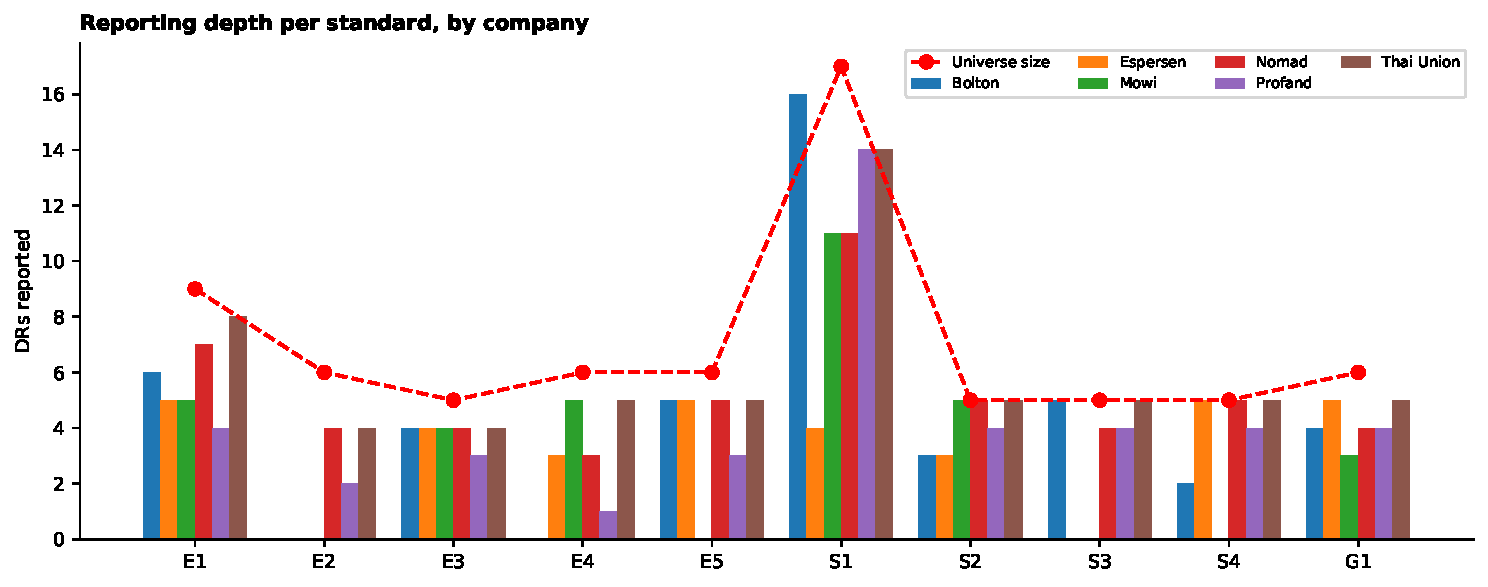
\includegraphics[width=\linewidth]{phase1/p1_depth_per_standard.pdf}
\caption{Reporting depth per topical standard, by company (bars), against
the number of screened DRs in each standard (red line). The gap between
the bars and the red line is widest for E2 (pollution) and E4
(biodiversity), the sector's thinnest topics.}
\label{fig:p1-depth}
\end{figure}

\textbf{What frequency does and does not mean.} One caveat governs the reading of
this funnel: it measures \emph{reporting convention} among large, mostly
CSRD-scoped reporters, not materiality for a small processor. A frequently
reported requirement is one an SME is likely to be \emph{asked about} as that
convention cascades down the value chain - a demand-relevance proxy - rather
than a topic asserted to be material for any individual firm. Whether these
revealed priorities fit a particular firm's situation is a separate question,
taken up in the cross-framework mapping and the worked case that follow.

\FloatBarrier
\subsection{5.4 The height of the frontier: a coverage
gradient}\label{cohort-gradient}

Coverage ranges from 33 to 60 of the 70 screened DRs
(Figure~\ref{fig:p1-heatmap}). Thai Union is the deepest reporter
at 60 DRs (86\%), followed by Nomad Foods (52; 74\%) and Bolton (45;
64\%); the median large reporter covers roughly 44 DRs, around 63\% of the
70-DR universe.
The immediate and consequential observation is that
\emph{even the frontier is incomplete}: the most advanced reporter in the sector
leaves around one relevant requirement in four uncovered (roughly 25 per cent),
and the median large reporter closer to two in five (around 40 per cent). If the
sector's most
resourced firms do not disclose the full set of relevant requirements, the
realistic ceiling for a resource-constrained SME sits well below
completeness - a point that reframes the SME question from 'how do we
report everything?' to 'which subset matters most?', which the demand
mapping in the following chapters answers.

The company-by-standard heatmap also shows that firms specialise: Bolton
reports most fully on own-workforce disclosure (S1, 16 of 17) and affected
communities (S3, 5 of 5); Espersen reports fewer S1 items (4 of 17) and no
S3 items in this coding, but is complete on consumers/end-users (S4, 5 of
5); Mowi's disclosure does not extend to affected communities (S3) or
consumers (S4) in this coding. The frontier is therefore not only
incomplete in height but uneven in shape from firm to firm.

\begin{figure}[htbp]
\centering
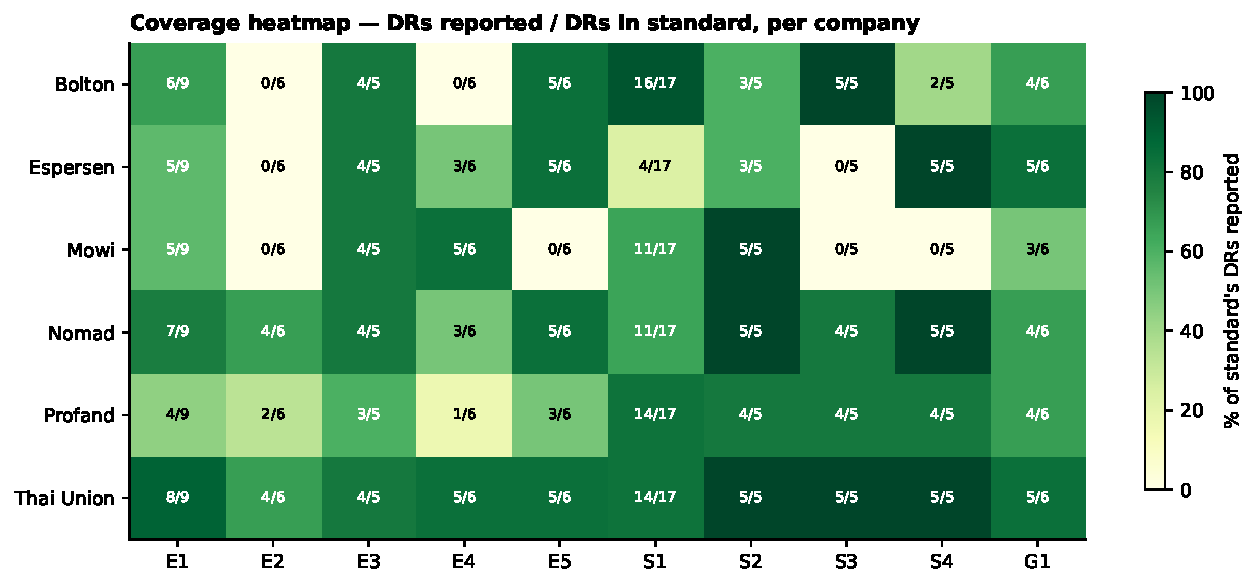
\includegraphics[width=\linewidth]{phase1/p1_heatmap.pdf}
\caption{Coverage heatmap: each cohort firm's reported DRs as a fraction
of the screened DRs in each of the ten topical standards (cell label
``reported / in standard''; shading is the percentage). Rows sum to each
firm's total in Table~\ref{tab:cohort-r}; the standard totals sum to the 70
screened DRs.}
\label{fig:p1-heatmap}
\end{figure}

\FloatBarrier
\subsection{5.5 The universal core: what every firm
reports}\label{cohort-core}

Beneath the gradient lies a stable core. Reading the universe by the
number of firms reporting each requirement produces a clean funnel: of the
63 DRs reported by at least one firm, 28 are reported by at least five, and
13 by \emph{all six} (Figure~\ref{fig:p1-frequency-r}). These 13 requirements are
the sector's empirically revealed \emph{baseline} - the disclosures every mature
reporter makes irrespective of sourcing model, and so, on the reading above, the
minimum a credible seafood reporter is now taken to be expected to cover. They
fall into four blocks:

\begin{itemize}
\item \textbf{Climate (3):} energy consumption and mix (E1-5), gross
  Scope~1--3 and total GHG emissions (E1-6), and climate targets (E1-4).
\item \textbf{Water (3):} actions and resources (E3-2), targets (E3-3),
  and water consumption (E3-4).
\item \textbf{Governance (2):} business-conduct policies and corporate
  culture (G1-1), and prevention and detection of corruption and bribery
  (G1-3).
\item \textbf{Social (5):} own-workforce policies (S1-1), workforce
  characteristics (S1-6), health-and-safety metrics (S1-14), and, for
  value-chain workers, policies (S2-1) and remediation channels (S2-3).
\end{itemize}

This narrowing is the core descriptive finding of the chapter: the sector
does not disclose evenly across a broad front, but converges onto a compact,
shared backbone.

One qualification bounds these two counts. Seven of the 70 requirements cannot be
reported by more than three firms, because the GRI-ESRS bridge offers no route to
them and half the cohort is coded through GRI indexes (Section~5.3). Six of those
seven are reported by no firm at all, so the qualification binds on a single
requirement: E1-1, the climate transition plan, which could in principle reach
five of six were all three GRI-indexed firms to disclose one. The core of 13 is
unaffected either way, since none of the seven could reach six of six.

\begin{figure}[htbp]
\centering
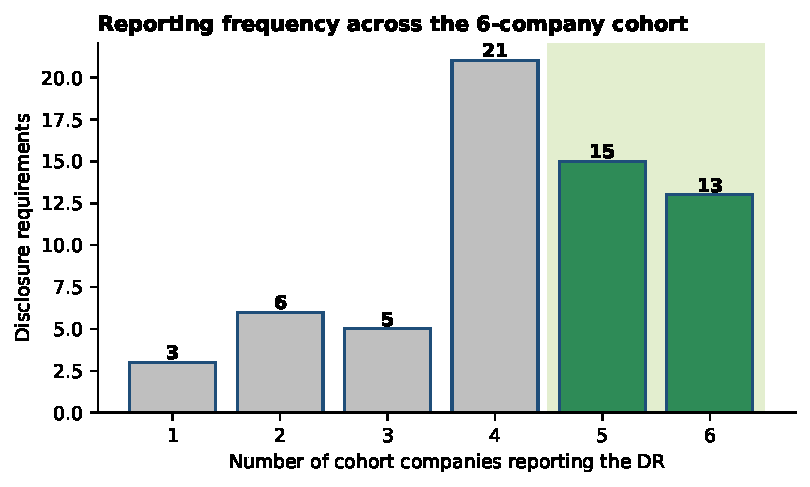
\includegraphics[width=0.8\linewidth]{phase1/p1_frequency.pdf}
\caption{Number of cohort firms reporting each DR, over the 63
requirements reported by at least one firm. The highlighted band (reported
by five or six firms) contains 28 requirements, of which 13 are reported
by all six - the universal core.}
\label{fig:p1-frequency-r} % RUBEN: overlaps fig:p1-frequency in Methodology 4.3 — same figure in both.
\end{figure}

\FloatBarrier
\subsection{5.6 The shape of the frontier: volume, consistency, and blind
spots}\label{cohort-shape}

Among the 63 reported requirements, disclosure is markedly social-heavy by
volume: 32 are Social, 26 Environmental, and 5 Governance, with the
own-workforce standard (S1) alone accounting for 17. This social weighting
holds within firms as well as across the universe: for every cohort
member, Social is the largest block of reported DRs and Governance the
smallest (Figure~\ref{fig:p1-esg}, panels~A--B). This is a volume comparison,
however, and the ESRS universe itself is uneven across pillars - 32 DRs each
for Environmental and Social, but only 6 for Governance. Normalized by each
pillar's own size (Figure~\ref{fig:p1-esg}, panel~C), Governance is in fact
the \emph{most} thoroughly covered pillar per firm on average (mean 69\% of
its 6 DRs, range 50--83\%, against a mean 56\% for Environmental and 70\% for
Social): the sector reports on a smaller
absolute footprint of governance topics not because it neglects them, but
because the ESRS asks fewer governance questions to begin with.

Volume, however, is not the same as consensus. Measuring each topic by the
mean number of firms reporting its requirements reveals where the sector
genuinely agrees (Figure~\ref{fig:p1-consistency}): consistency is highest for
water (E3, mean 5.75 of 6), value-chain workers (S2, 5.00), governance (G1,
5.00) and resource use and waste (E5, 4.60), and lowest for pollution (E2,
2.50), biodiversity (E4, 3.40) and affected communities (S3, 3.60).
The frontier is thus concentrated on water, workforce, governance and
resource-use topics and thins markedly across pollution, biodiversity and
community disclosure.

The seven requirements reported by no firm sharpen this picture, though they
need careful reading. Four are the ``anticipated financial effects''
disclosures - for pollution (E2-6), water (E3-5), biodiversity (E4-6)
and circular economy (E5-6) - the forward-looking, financially
quantified requirements that are the most demanding and are phased in under
the standards. The remaining three are substances of concern (E2-5),
internal carbon pricing (E1-8) and payment practices (G1-6). The sector's clearest collective gap is therefore
the financial quantification of environmental impact, followed by
pollution disclosure - a pattern consistent with the low consistency of E2
across the cohort.

One qualification applies before this is read as a sector-wide finding. Six of
the seven have no route through the GRI-ESRS bridge, so for the three GRI-coded
firms they were screened directly in the report bodies rather than through the
index (Section~5.3); none was found. The absence is therefore observed for all
six firms rather than inferred, but by two different instruments. A second point
is substantive: the
anticipated-financial-effect requirements are phased in under the ESRS on a
delayed timeline, so their absence reflects current transitional relief as much as
a genuine reporting gap - they are not yet required, rather than being avoided. A parallel movement appears
in materiality itself: across 241 large listed EU companies, Nahrstedt (2026)
finds double-materiality assessments declaring fewer topics material between
FY2024 and FY2025, the decline concentrated in the environmental standards other
than climate. Firms are not only disclosing less here, they are increasingly
judging these topics immaterial - consistent with a landscape still calibrating
rather than one that has settled.

\begin{figure}[htbp]
\centering
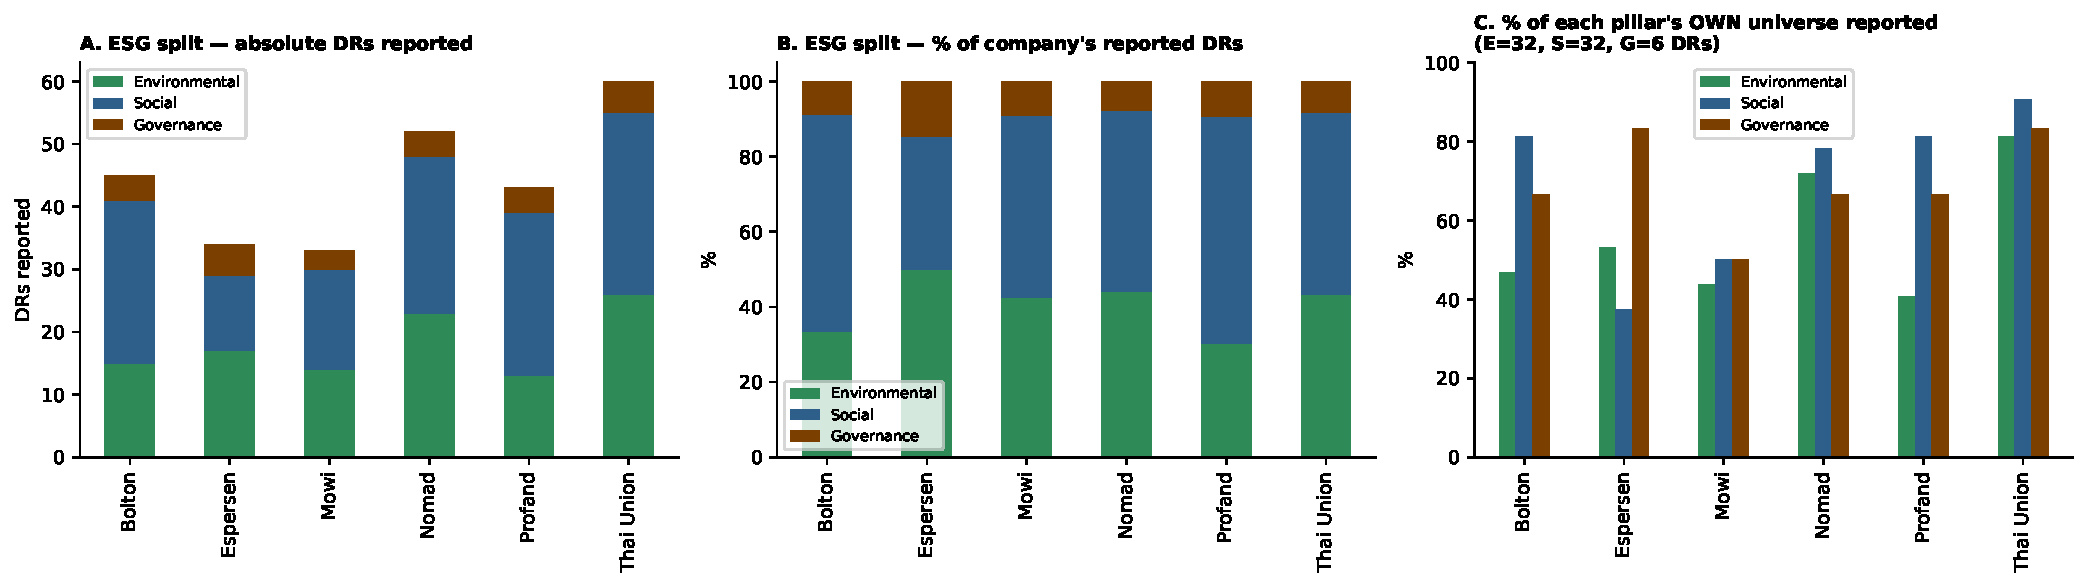
\includegraphics[width=\linewidth]{phase1/p1_esg_split.pdf}
\caption{ESG composition of each firm's reported DRs: in absolute terms
(panel~A), as a share of the firm's total reported DRs (panel~B), and as a
share of each pillar's own ESRS universe - 32 DRs each for Environmental
and Social, 6 for Governance (panel~C). By volume, Social is the largest
block and Governance the smallest for every firm (A--B); normalized by
pillar size, Governance is the most thoroughly covered pillar (C).}
\label{fig:p1-esg}
\end{figure}

\begin{figure}[htbp]
\centering
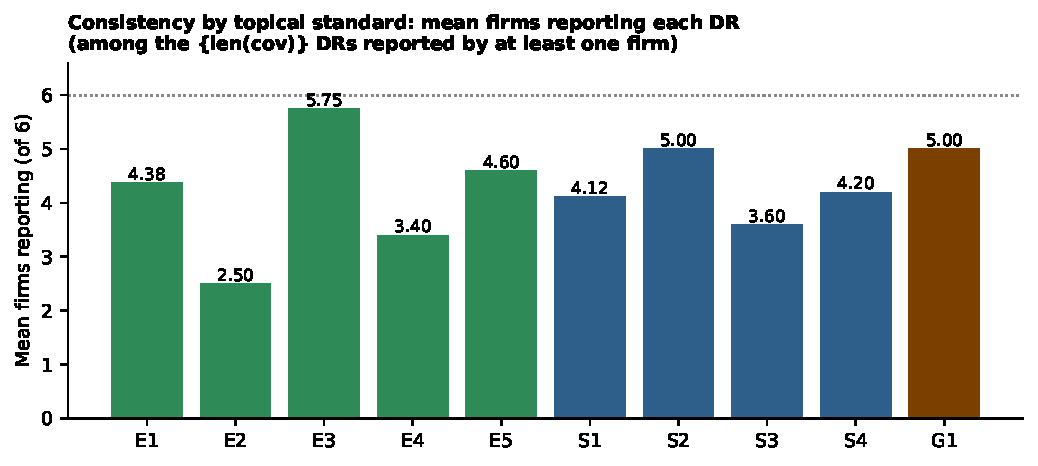
\includegraphics[width=0.75\linewidth]{phase1/p1_consistency.pdf}
\caption{Consistency by topical standard: mean number of cohort firms
reporting each DR, among the 63 DRs reported by at least one firm.
Consistency is highest for water (E3) and governance (G1); lowest for
pollution (E2) and affected communities (S3).}
\label{fig:p1-consistency}
\end{figure}

\FloatBarrier
\subsection{5.7 Robustness across sourcing models and reporting
year}\label{cohort-robustness}

\textbf{Does the core depend on sourcing model?} Because the cohort deliberately
spans four sourcing models, the universal core can be tested for whether it is an
artefact of one type of firm. It is not: the 13 core requirements are reported
across all four sourcing models - wild-capture, aquaculture, integrated
wild-plus-aquaculture, and diversified multi-species sourcing alike. All six
firms remain seafood \emph{processors} throughout; what varies between the four
groups is only what and how each sources - not whether processing is what
they do. Sourcing model changes only the \emph{edges} of the
picture, not the centre: model-specific topics such as feed and animal health
(aquaculture) or wild-stock status (wild-capture) appear only in the long tail,
while the climate, water, governance and workforce core is common to all. This
is confirmed rather than merely illustrated: because these 13 requirements are
by definition reported by \emph{all six} cohort firms, every sourcing-model
subgroup necessarily reports them too - there is no possible split by which
they could fail to be cross-model.

Two further checks confirm the core is not an artefact of the sample. First,
\emph{threshold sensitivity}: the near-universal set contracts smoothly with the
cut - 60 requirements are reported by at least two firms, 54 by at least three,
49 by at least four, 28 by at least five, and 13 by all six - so the $\geq$5-of-6 line sits on a gradient rather than a
cliff edge: the shortlist shrinks smoothly as the threshold tightens, with no
sharp jump at any single cut, so the choice of $\geq$5-of-6 is not an arbitrary
point that the result hinges on. Second, \emph{cohort-size invariance}: re-deriving the near-universal
set on the five European firms alone, dropping the non-European Thai Union at the
equivalent $\geq$4-of-5 cut, returns the \emph{identical} 28-requirement set - a
complete overlap, so the backbone does not depend on which firms are in the
cohort (Figure~\ref{fig:p1-cohort-invariance}).
Thai Union itself, the single non-EU firm and the broadest reporter (60 of
70), reports \emph{more} widely on biodiversity, affected communities and
pollution than the European average. This thesis does not investigate why
that pattern holds, and no assumption about its cause, whether GRI's broader
reporting scope, company-specific policy, or any other factor, is made here;
the observation is reported descriptively and left at that. What matters here is only that one requirement is reported
uniquely by Thai Union, so the consensus core survives the EU/non-EU divide
as common ground rather than an EU-regulatory artefact. In short, the same 13-topic core emerges whichever way the cohort is cut
- by the reporting threshold, by which firms are included, and by EU versus
non-EU - which is what lets it be read as a genuine feature of the sector rather
than a quirk of this particular sample.

\begin{figure}[htbp]
\centering
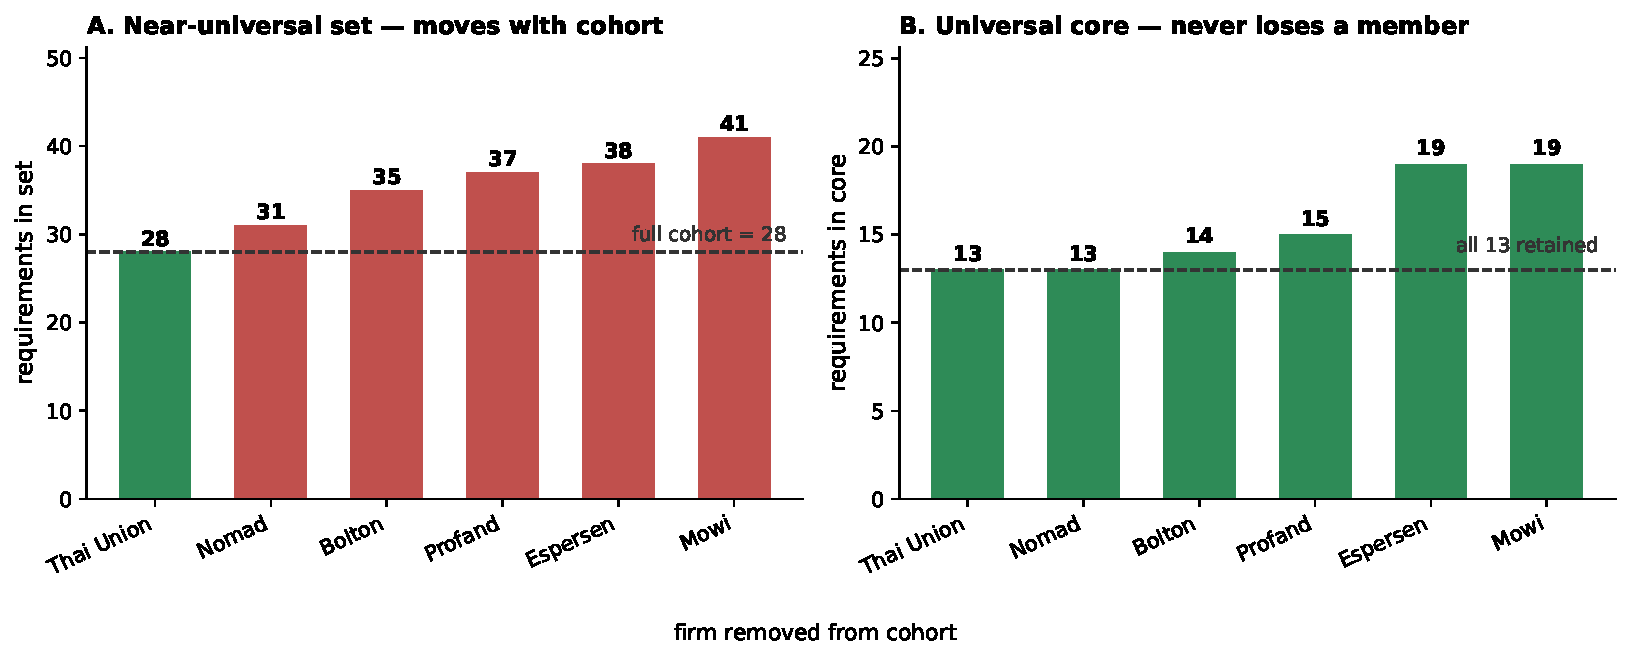
\includegraphics[width=0.7\linewidth]{phase1/p1_cohort_invariance.pdf}
\caption{Cohort-size invariance: the near-universal set (28 DRs) is
identical whether derived from the full six-firm cohort at the
$\geq$5-of-6 threshold or from the five European firms alone at the
equivalent $\geq$4-of-5 threshold.}
\label{fig:p1-cohort-invariance}
\end{figure}

Finally, an \emph{exploratory} observation, not a statistical result. The cohort
mixes 2024 and 2025 reporting years, and for the three firms with two comparable
years reported coverage was flat or fell very slightly - Nomad Foods from 53 to 52
DRs, Profand unchanged at 43, and Espersen from 36 to 34 - driven by a handful of
requirements dropped and none added (Figure~\ref{fig:p1-year}). With only
three firms over two years, no weight can be placed on this beyond its direction;
the main analysis uses each firm's most recent report (the figures in
Table~\ref{tab:cohort-r}). It runs against the
assumption of ever-expanding disclosure, and a comparable direction appears at
scale. The first large-scale longitudinal study of double-materiality outcomes
under the CSRD, covering 241 large listed EU companies, finds materiality rates
declining moderately between FY2024 and FY2025, concentrated in the
environmental standards other than climate (Nahrstedt, 2026). That study measures
which topics firms judge \emph{material}, not how much they disclose, so it is a
parallel indicator rather than a direct comparison; the two nonetheless move the
same way. The discussion returns to this under the Omnibus simplification.

\begin{figure}[htbp]
\centering
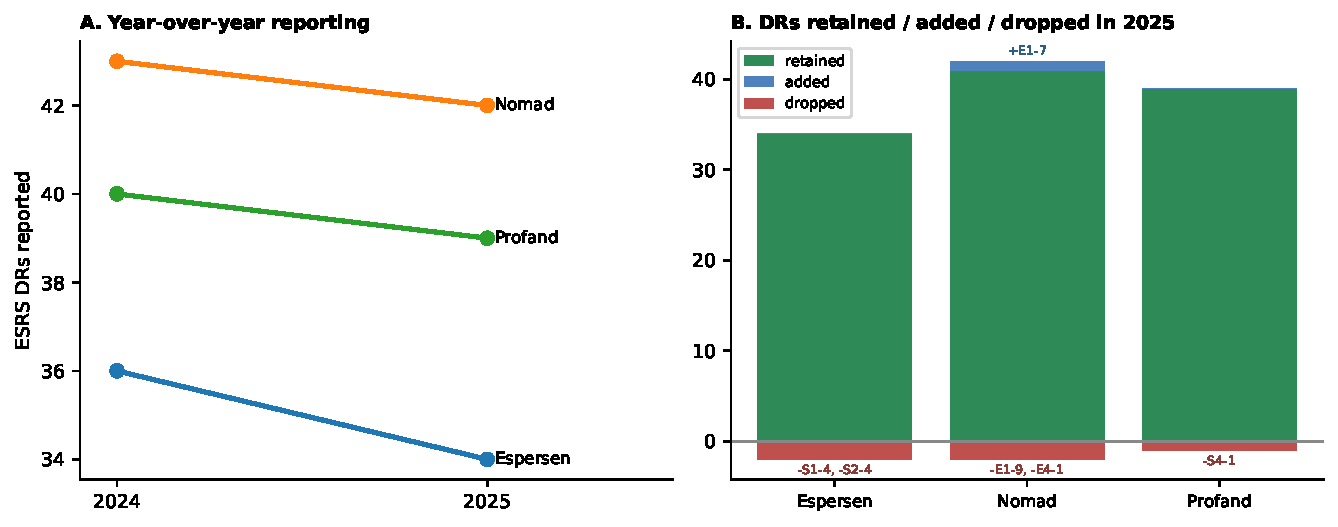
\includegraphics[width=\linewidth]{phase1/p1_year_evolution.pdf}
\caption{Year-over-year reporting for the three firms with both a 2024 and
a 2025 report. Panel~A: total DRs reported, which fell for all three.
Panel~B: requirements retained, added and dropped in 2025 - change is
dominated by retention, with a small net reduction.}
\label{fig:p1-year}
\end{figure}

\FloatBarrier
\subsection{5.8 What the cohort establishes - and what it does
not}\label{cohort-limits}

The cohort establishes three things. It fixes the height of the sector's
disclosure frontier at 53 requirements for the deepest reporter and around
57\% of the screened set for the median large firm; it identifies a
13-requirement universal core spanning climate, water, governance and
workforce that constitutes the sector's de facto baseline expectation; and it
locates the sector's collective gaps in the anticipated-financial-
effect and pollution requirements. Together these calibrate the realistic
disclosure ambition for a smaller firm and supply the empirical anchor for
the cross-framework demand mapping that follows.

\textbf{What this means for the SME question.} Read together, these findings do
more than describe the frontier; they bound the smaller firm's problem. Because
even the best-resourced reporters converge on a compact, cross-cutting backbone
rather than reporting everything, the SME's task is not to approximate an
ever-expanding frontier but to build a short, stable set of disclosures the sector
has already revealed to be expected - and that a firm is, on the
demand-relevance reading, most likely to be asked for. This is the hard
step described at the start of this chapter (Section~5.1); the
contribution here is to make it concrete for one sector by naming the
topics on which it should begin. That neither disclosure nor declared
materiality is expanding in the early CSRD years (Nahrstedt, 2026) only
strengthens the case for a proportionate, prioritised starting point
over open-ended completeness. \emph{Which} of these topics an individual firm
should build first, given the specific demands it faces, is the question the
cross-framework mapping takes up next.

Its limits are equally definite and are stated so that the findings are
not read beyond what they support. The cohort is a purposive sample of six
upper-bound reporters and is not representative of the sector, so no claim
about typical or average practice is made. Coverage is binary presence at
DR level and speaks to breadth, not to the depth, quality or assurance of
disclosure. The mapping from mixed ESRS and GRI source documents onto the
ESRS requirement set rests on analyst judgement, for which the member-checking
step described in Chapter~3 is a corroboration still outstanding rather than a
completed control. And the analysis is a 2024--2025 snapshot of a rapidly moving
reporting landscape. Within these
bounds, the cohort provides what it was designed to provide: a defensible,
document-grounded map of the seafood disclosure frontier.


% =====================================================================
